\section{Partición en clusters}

\begin{figure}
\centering
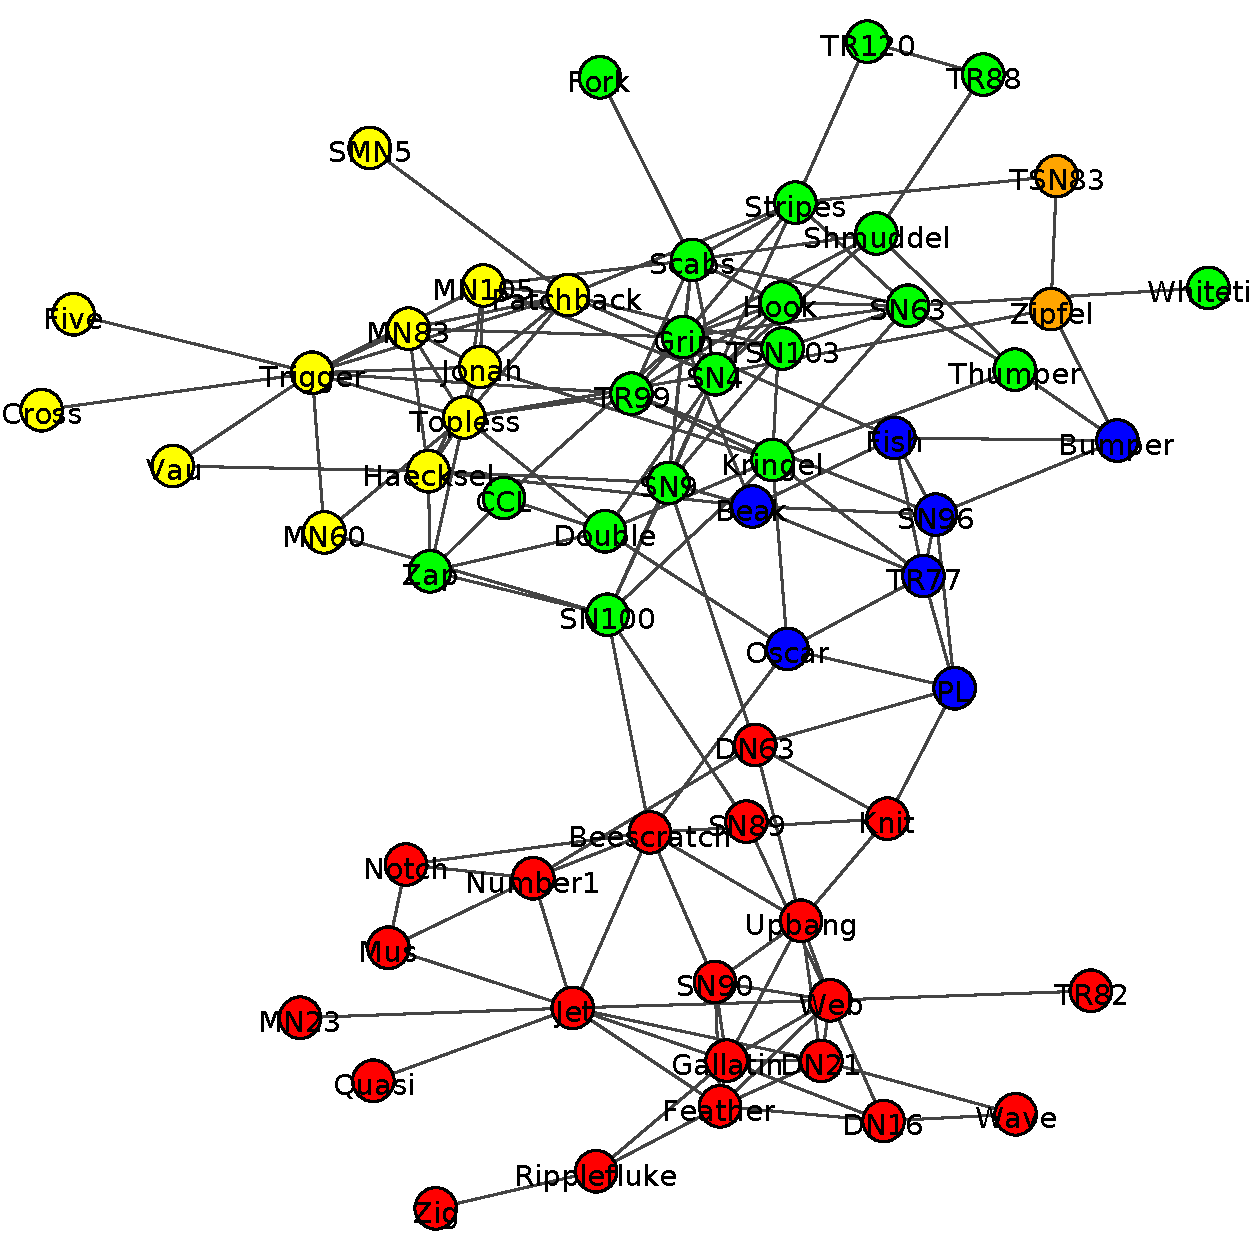
\includegraphics[scale = 0.2]{figuras/Edge_betweenness}
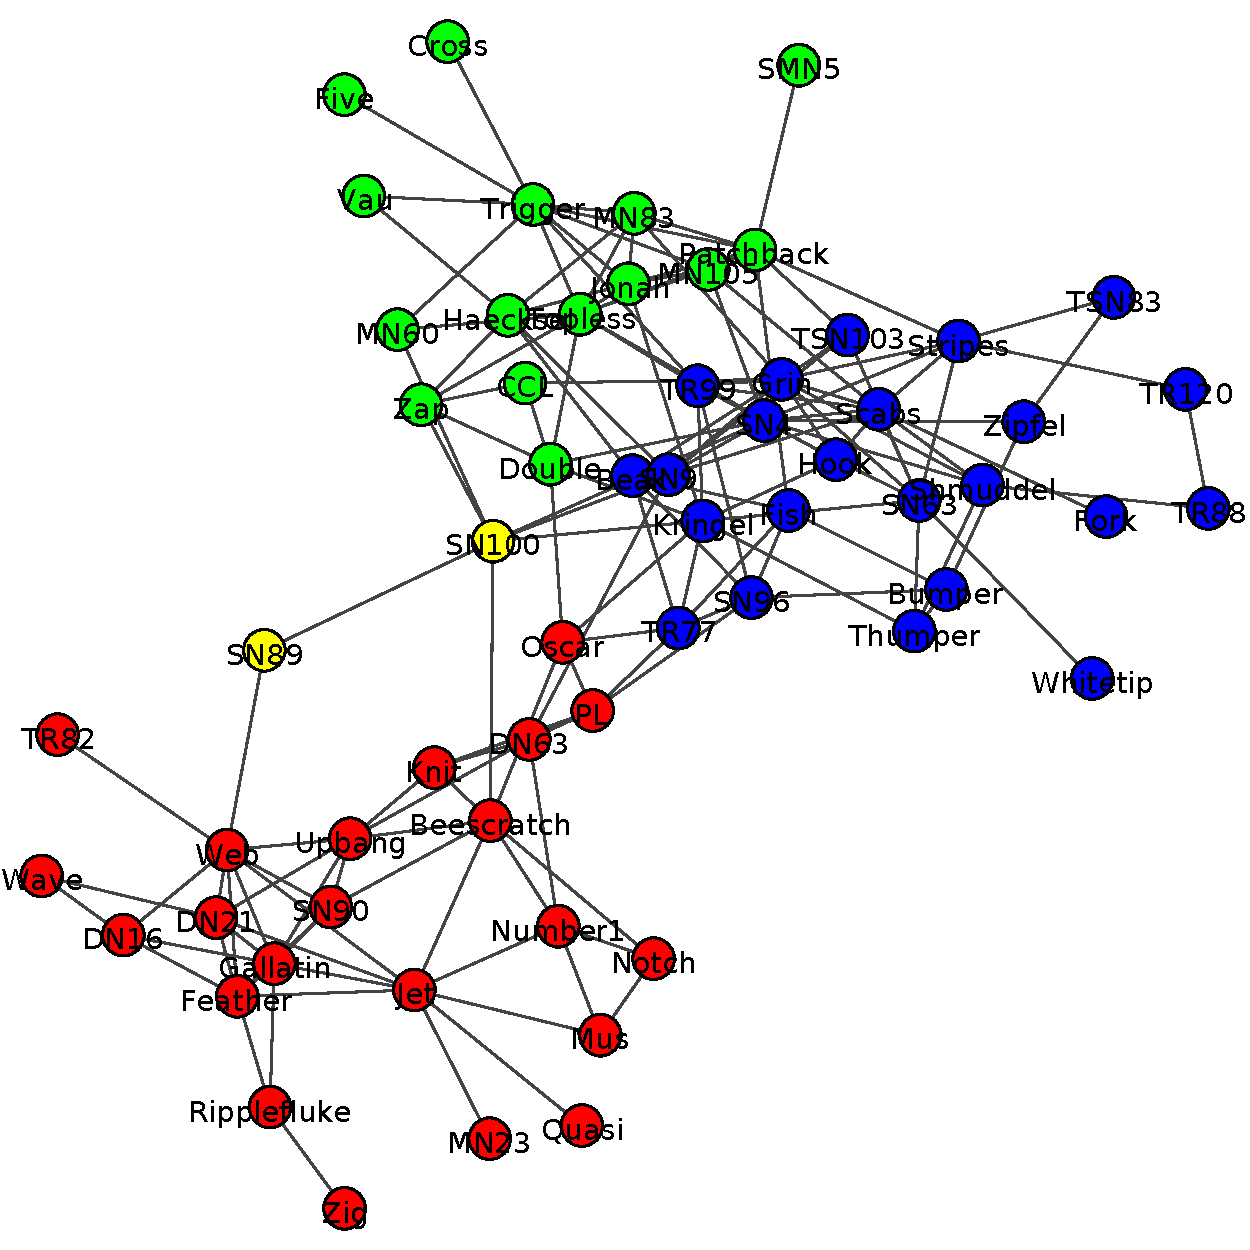
\includegraphics[scale = 0.2]{figuras/Fast_greedy} \\
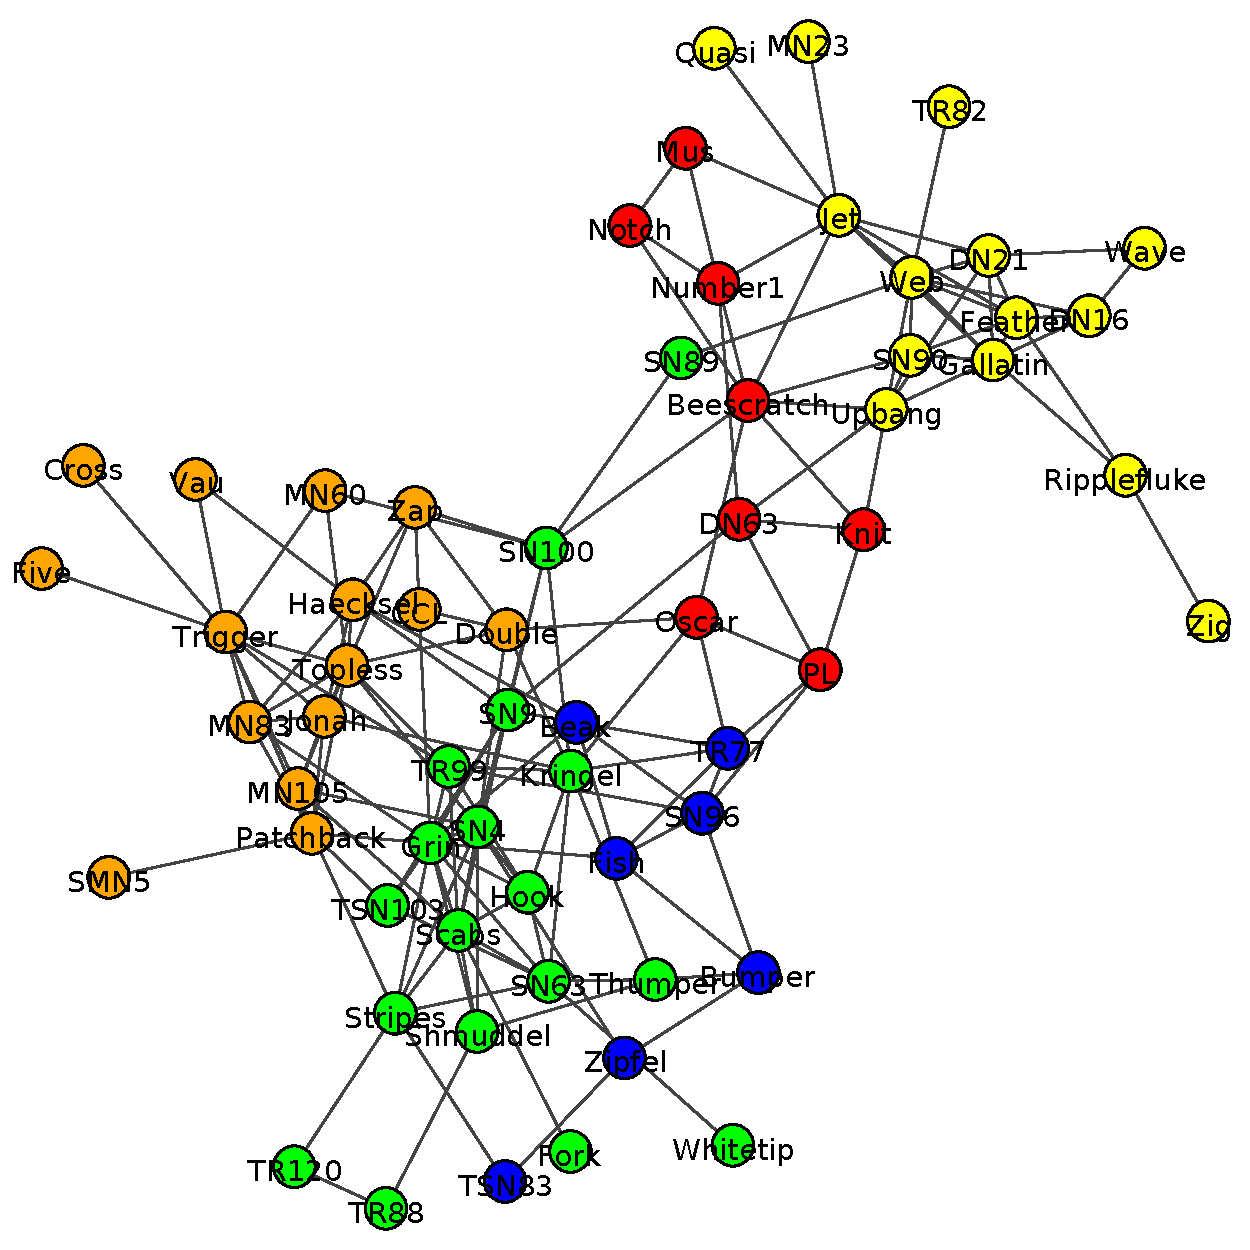
\includegraphics[scale = 0.2]{figuras/Louvain}
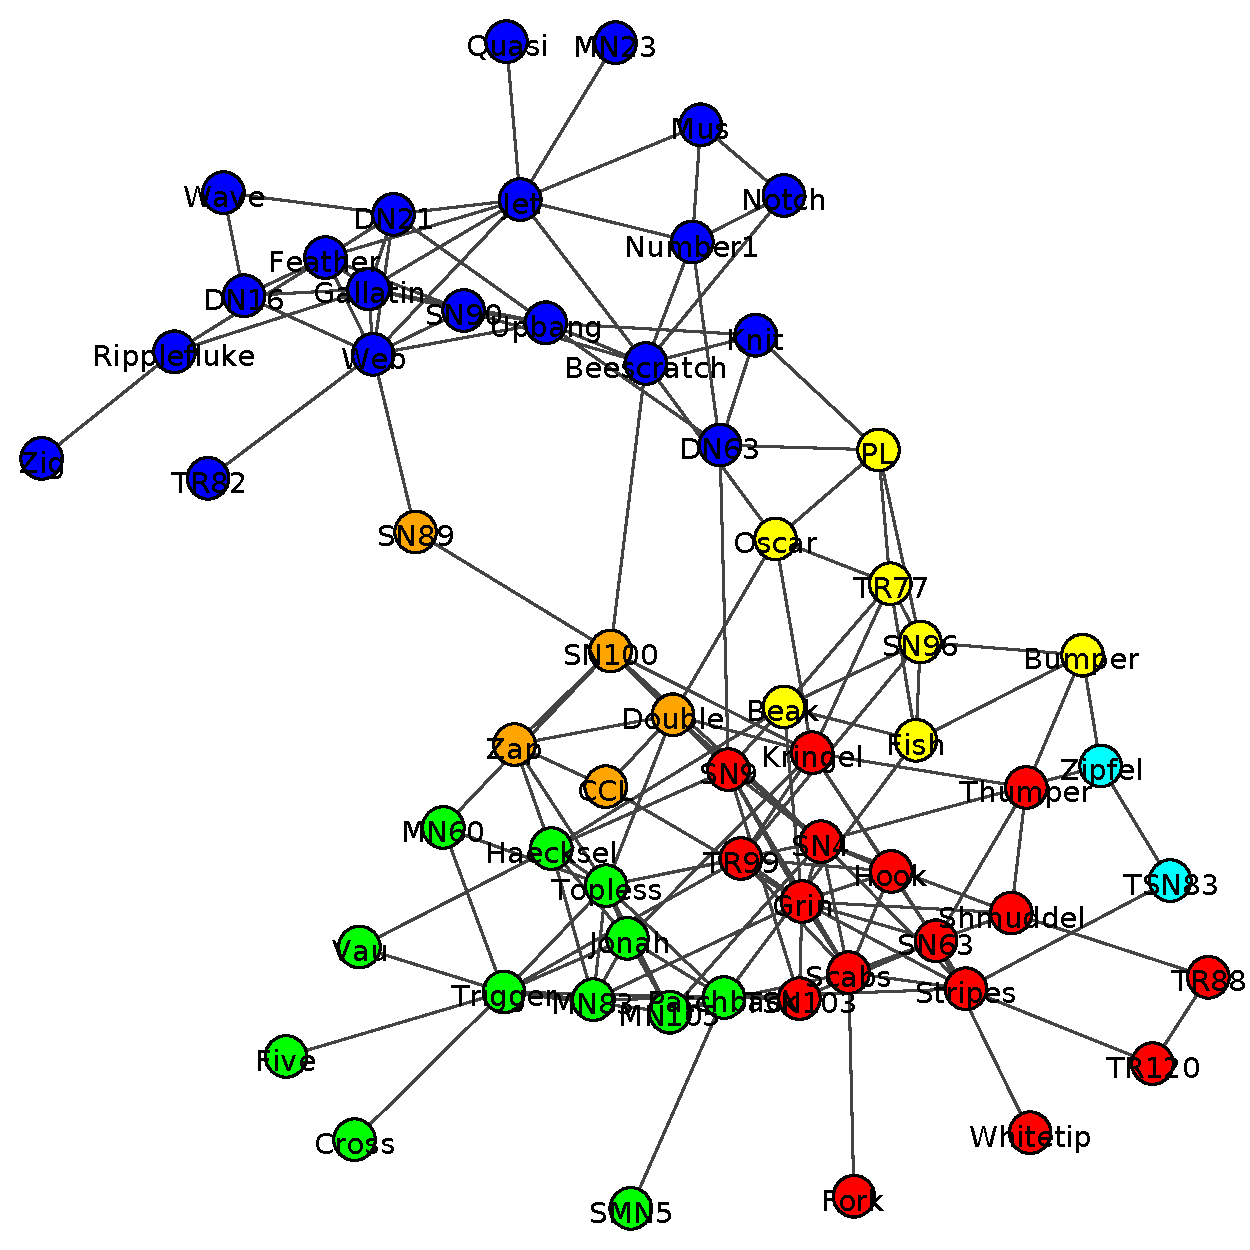
\includegraphics[scale = 0.2]{figuras/Infomap}
\caption{Layouts indicando el cluster asignado por cada algoritmo.}
\label{fig:Layouts_clusters}
\end{figure}

\section{Modularidad}

\begin{table}
\centering
\begin{tabular}{c c}
\hline \hline
Algoritmo & Modularidad \\
\hline
Fast greddy & 0.495 \\
Infomap & 0.529 \\
Edge-betweenness & 0.519 \\
Louvain & 0.519 \\
\hline\hline
\end{tabular}
\caption{Modularidad de las particiones dadas por diferentes algoritmos.}
\label{table:Modularidad}
\end{table}


\begin{figure}
\centering
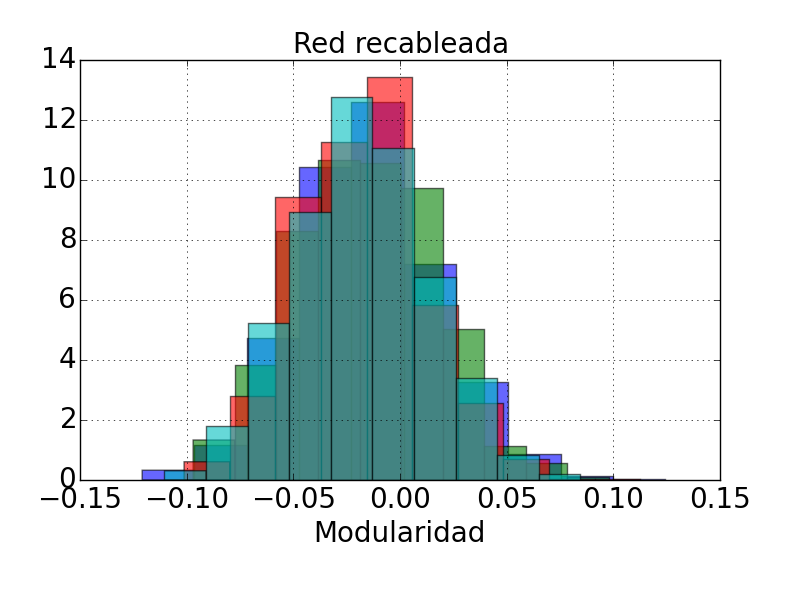
\includegraphics[scale = 0.5]{figuras/Modularidad_random}
\caption{Modularidad recableando en forma aleatoria, manteniendo la categoría dada por los algoritmos de detección de particiones.}
\label{fig:Modularidad_random}
\end{figure}
